\section{Final Bootware Architecture}
\label{design:finalarch}

\autoref{image:finalarchlocal} and \autoref{image:finalarchremote} show the final architecture of the local and remote bootware component.
Since the only difference between them is the provisioning engine plugin shown in the top right corner of \autoref{image:finalarchremote}, we will describe this figure only.
At the bottom we can see four exemplary event plugins.
These are loaded at the beginning of the bootware execution by the plugin manager, shown on the left of \autoref{image:finalarchremote}.
For demonstrations purposes, \autoref{image:finalarchremote} shows a wider range of possible event plugins.
All these plugins provide some sort of input and/or output mechanism for the bootware component.
A \nom{command-line interface}{CLI} plugin could be used to make the bootware operations accessible via a command-line interface.
A event logger plugin could be used to write all bootware events to a log file.
We can also imagine an event queue plugin that pushes all bootware events into some message queue, so that they can be consumed by other components.
Finally, an undeploy trigger plugin could trigger the undeployment of the bootware and all running payloads by listening for a specific message at the workflow middleware.
Besides the event plugins there is always the web service interface, shown at the bottom right of \autoref{image:finalarchremote}, which provides the standard way to interact with the bootware.

All event plugins and the web service interface work by implementing event handlers for certain events published at the event bus, or by publishing events to the event bus themselves.
As we can see in the center of \autoref{image:finalarchremote}, the event bus and the state machine form the core of the bootware.
The event bus is responsible for distributing events between the various plugins and the state machine.
The state machine implements the entire bootstrapping process, as described earlier in \autoref{design:flow}.
At certain points during the bootstrapping process, operations are delegated to the plugin manager to load plugins, and to the infrastructure, connection, payload, and provisioning engine plugins, shown at the top of \autoref{image:finalarchremote}.

\begin{figure}[!htbp]
	\centering
	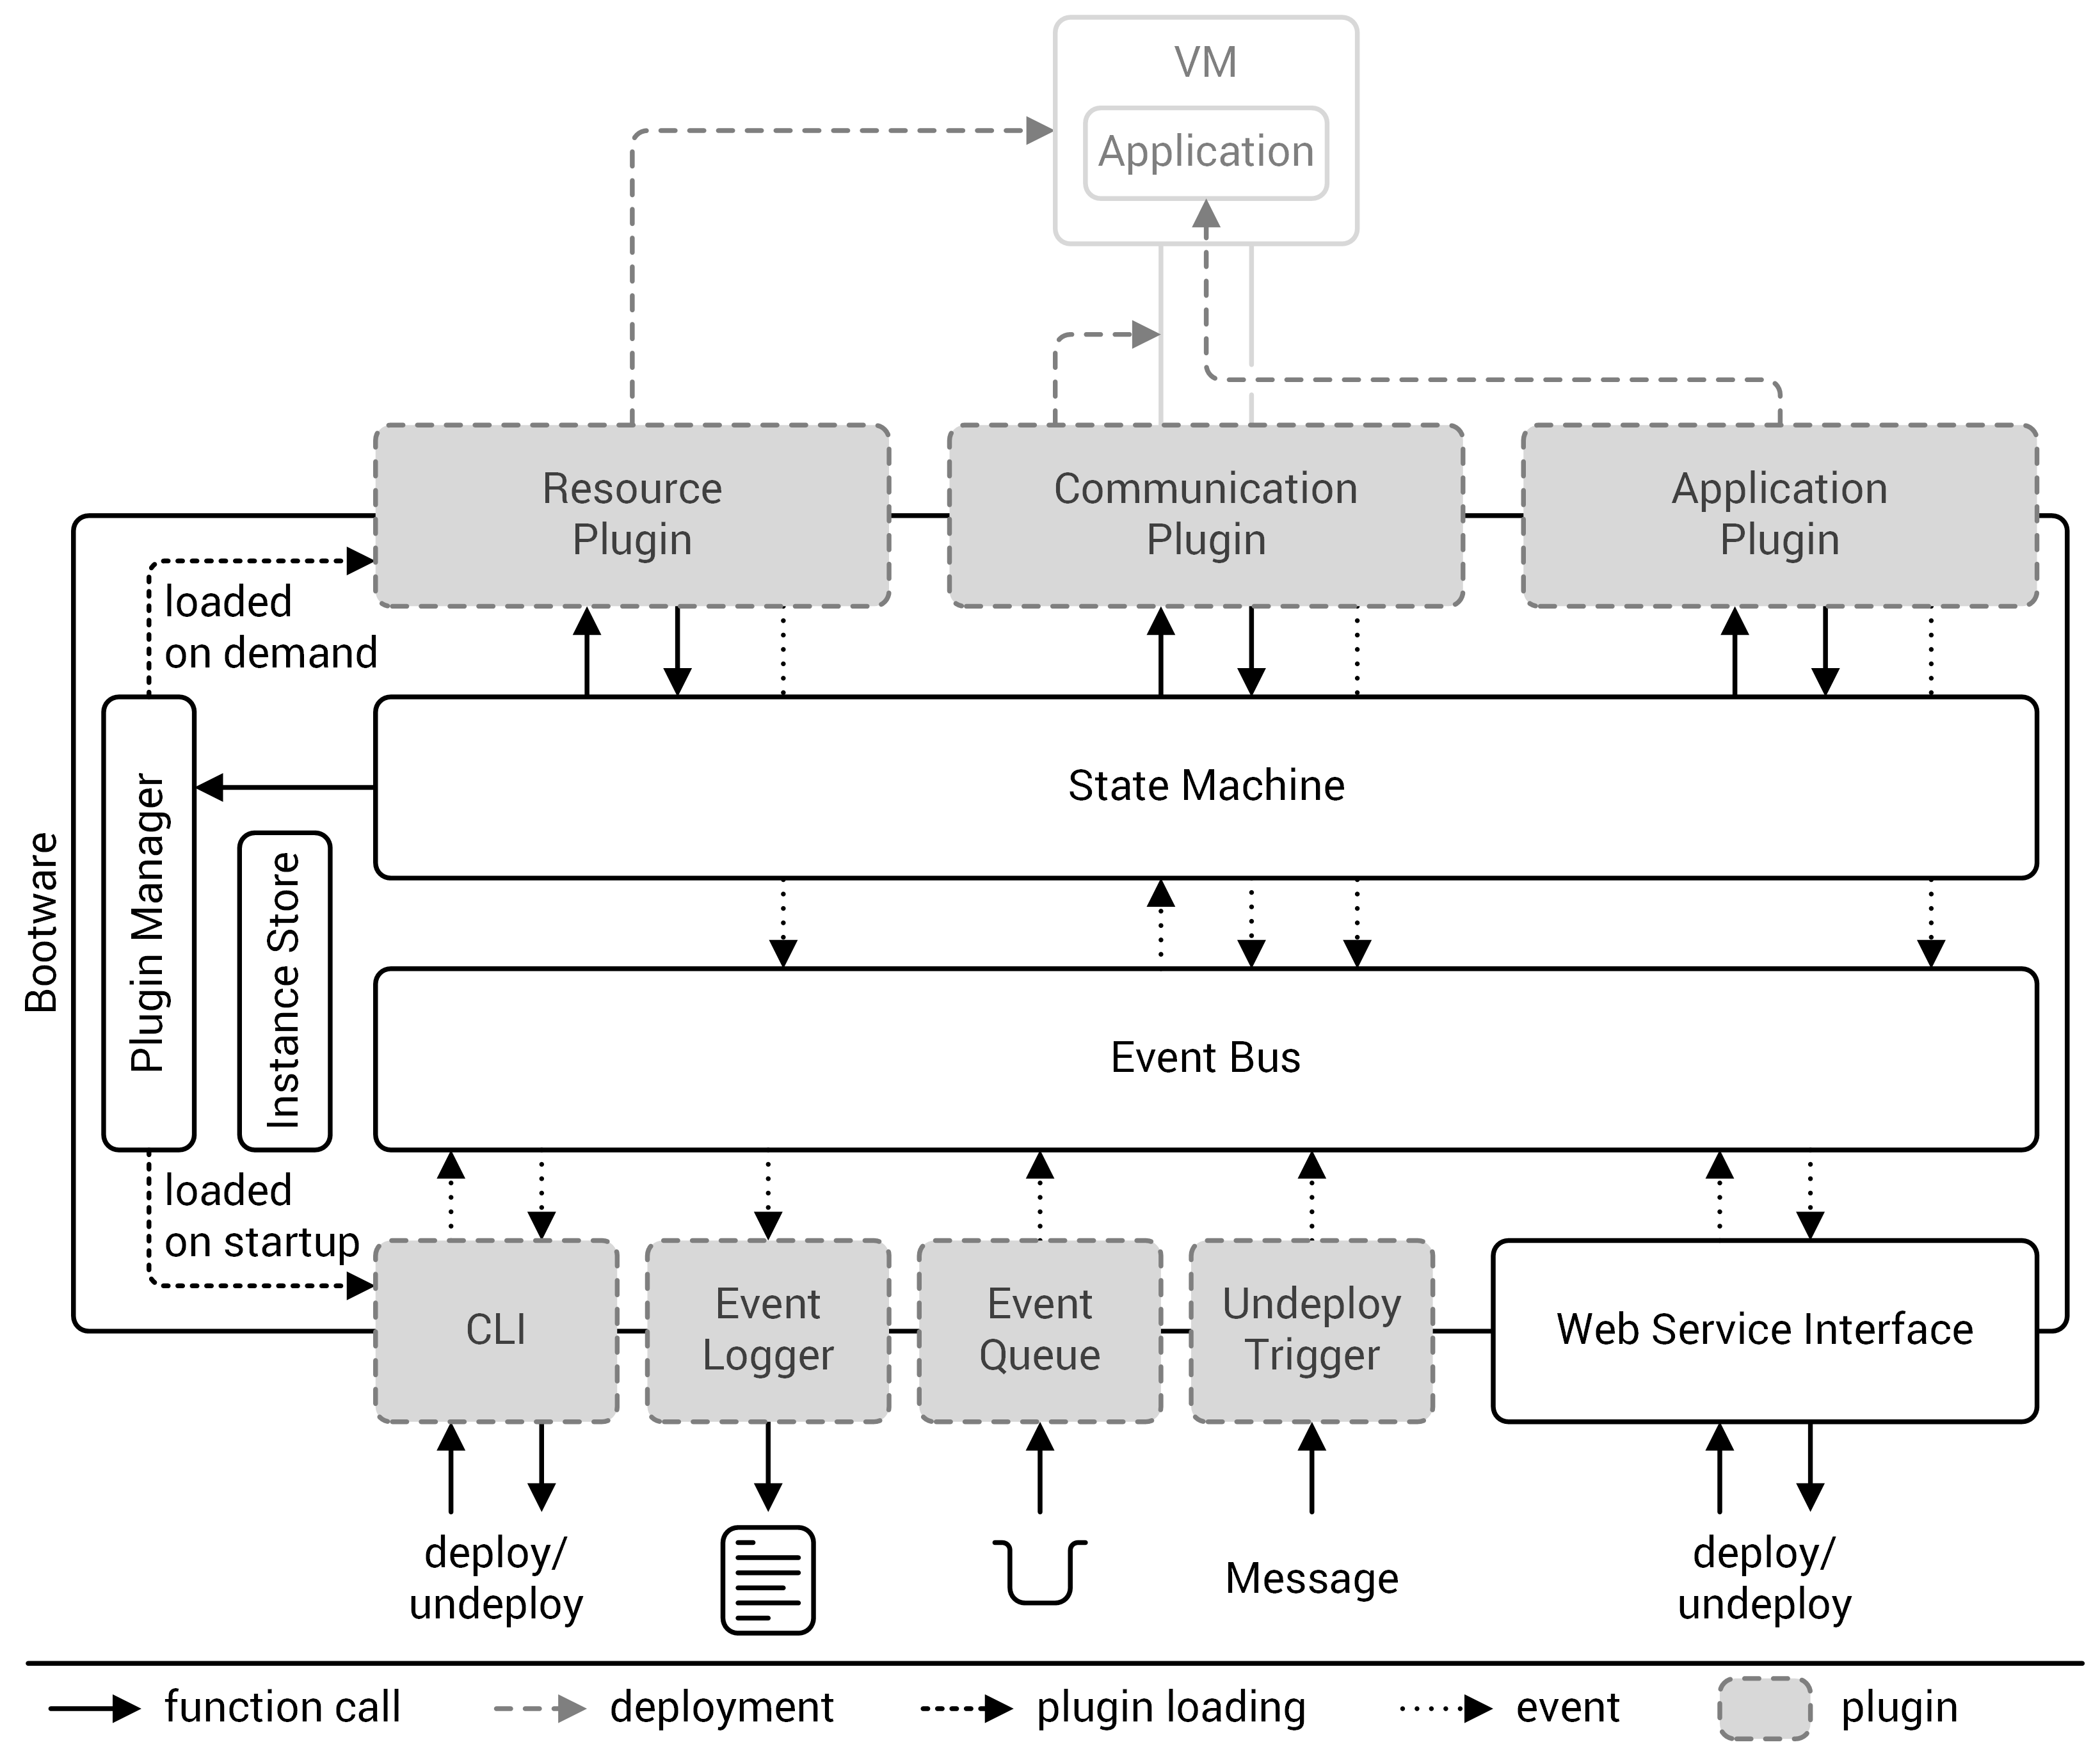
\includegraphics[resolution=600]{design/assets/final_architecture_local}
	\caption{The final architecture of the local bootware component.}
	\label{image:finalarchlocal}
\end{figure}

\begin{figure}[!htbp]
	\centering
	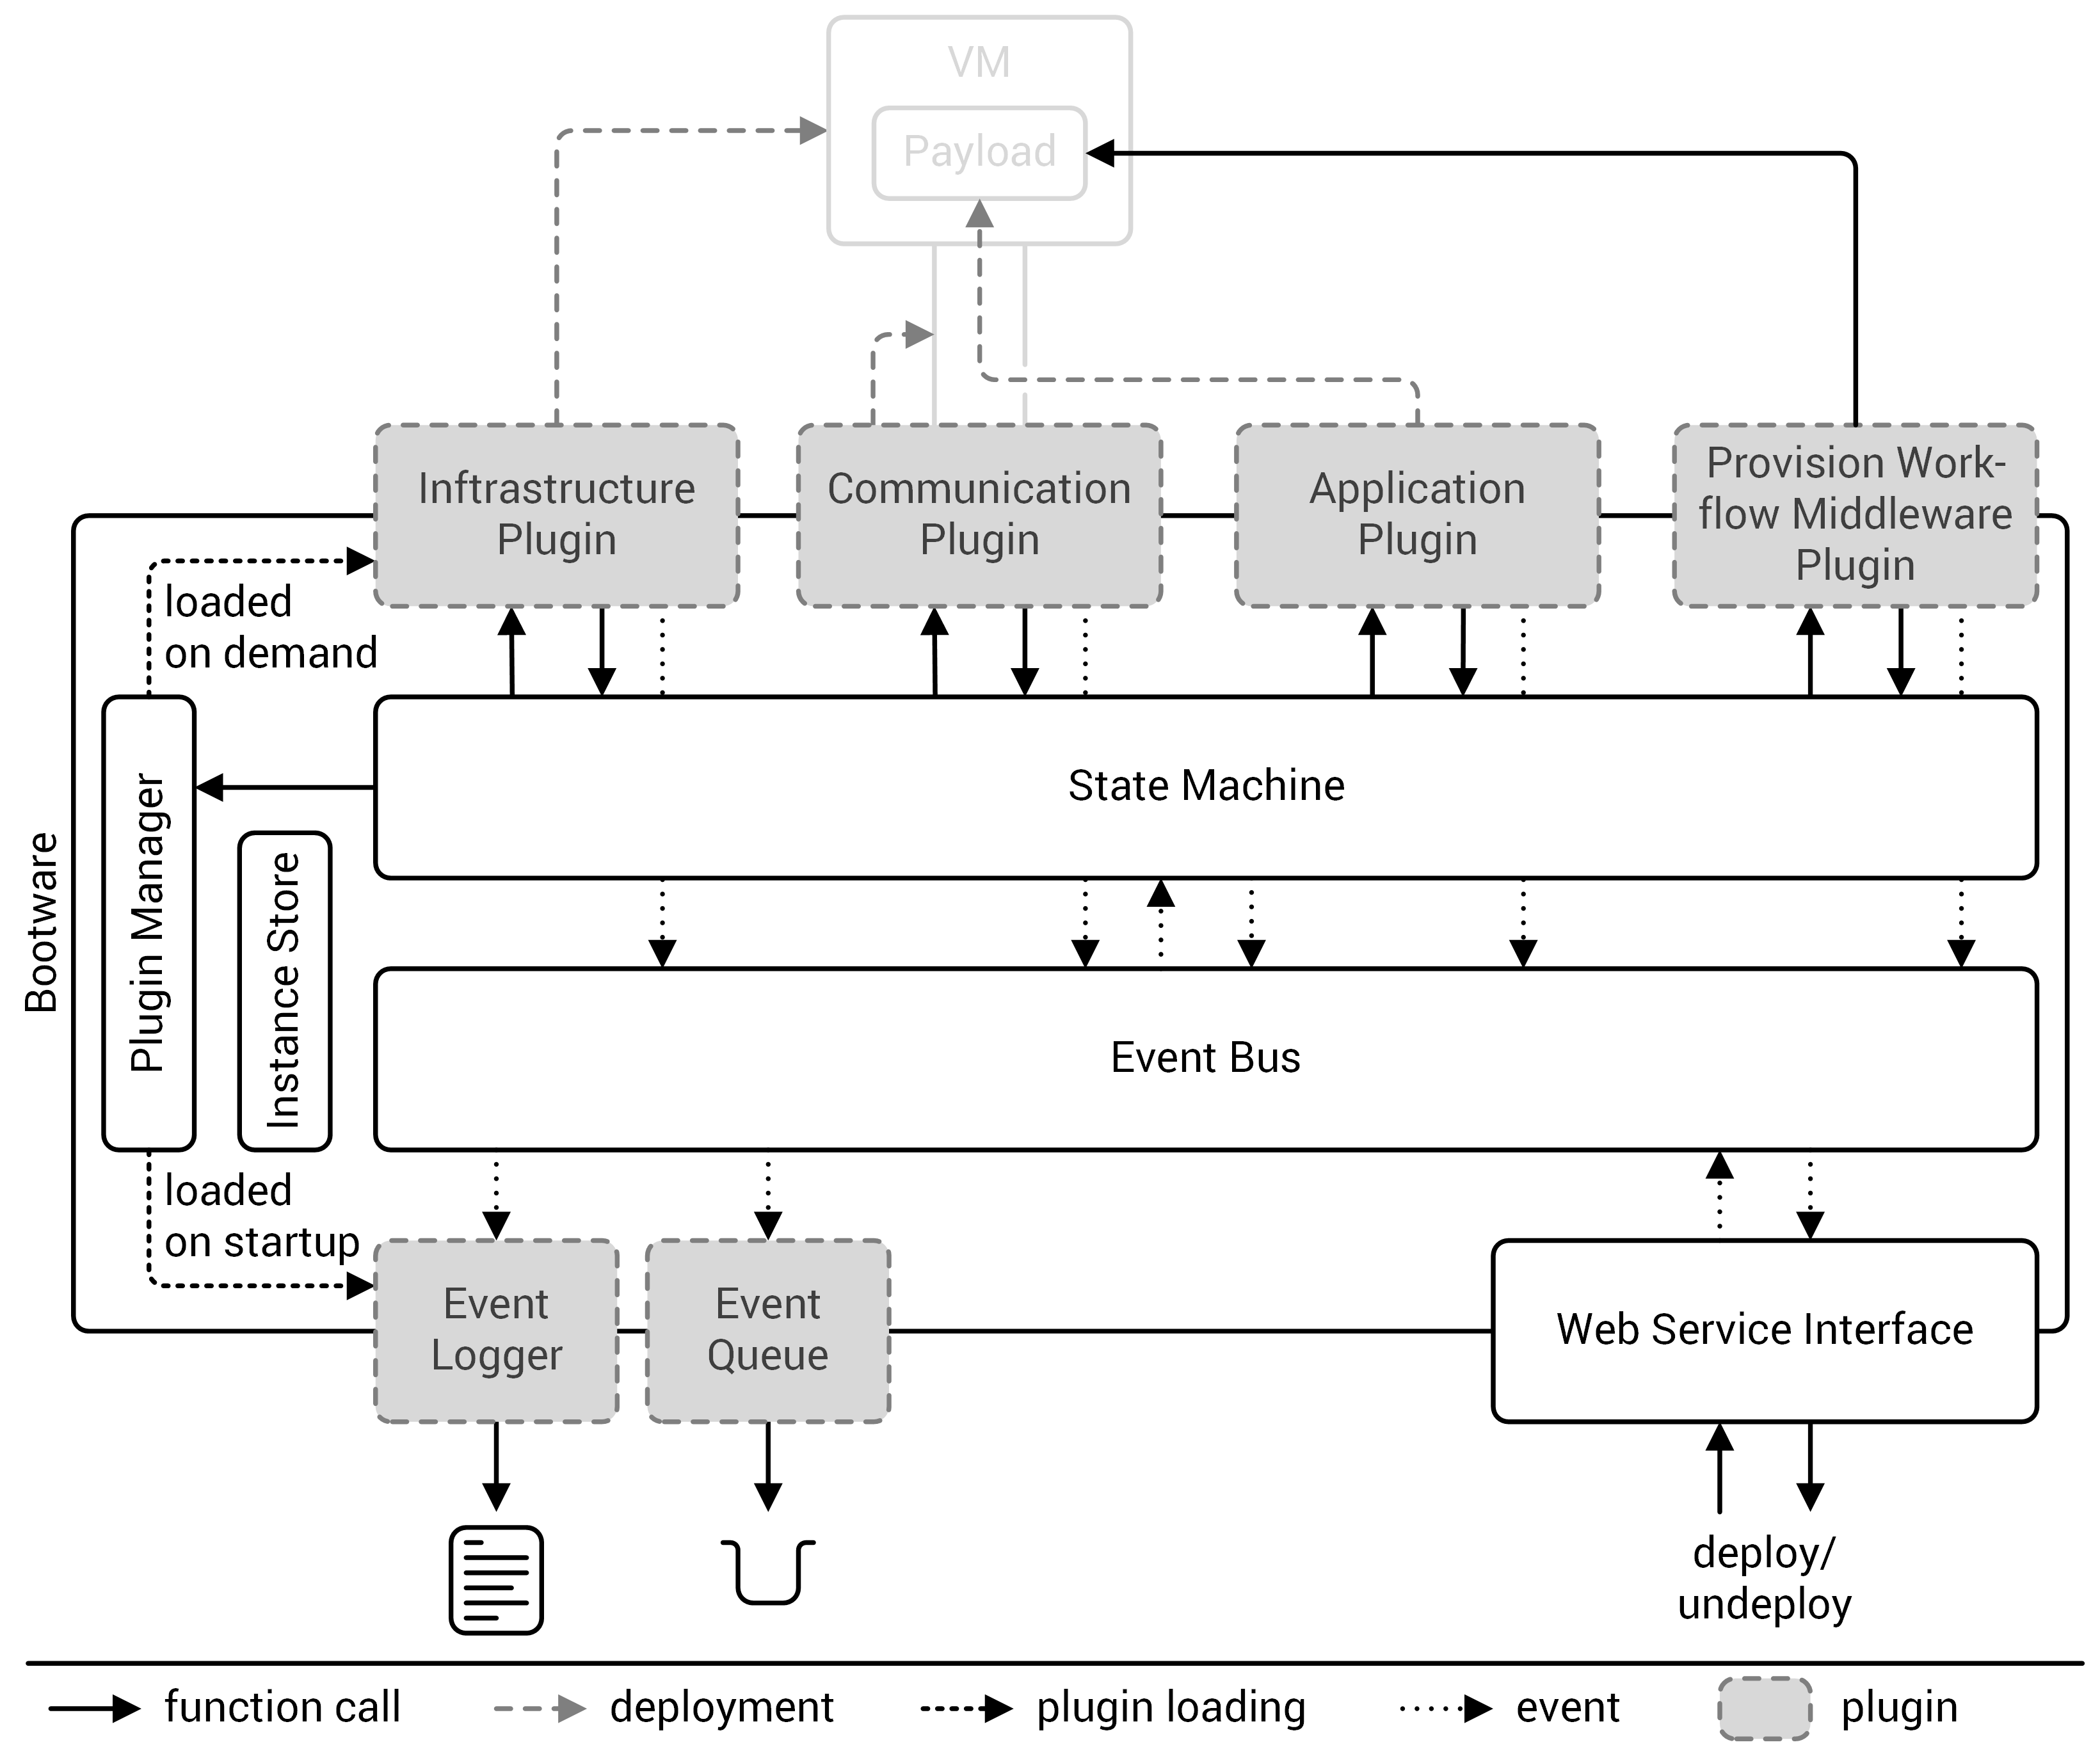
\includegraphics[resolution=600]{design/assets/final_architecture_remote}
	\caption{The final architecture of the remote bootware component.}
	\label{image:finalarchremote}
\end{figure}

The infrastructure, connection, and payload plugins implement the actual bootstrapping operations.
At the top, \autoref{image:finalarchremote} shows an exemplary result of these bootstrapping operations.
In this particular case, the infrastructure plugin started a VM, to which the connection plugin set up a communication channel.
The payload plugin then used this communication channel to provision the payload inside the VM.
The provisioning engine plugin is only available in the remote bootware and allows it to call a provisioning engine with the details necessary to provision the workflow middleware.
This is shown in \autoref{image:finalarchremote} as an additional function call from the provisioning engine plugin to the previously deployed payload.
During the bootstrapping procedure, events are sent from all these plugins back to the event bus to be delivered to the loaded event plugins.
